\subsection{Adding user management system}\label{subsec:user_management}

The old system didn't have a user management system, as it relied on the site being the
user so there wasn't really users to manage. So we had to integrate users within the system
then add a way to manage them, and this was done by migrating the site from being the user
to being an entity that could be managed by users who have the right to do so.
And that required rework through the majority of the backend as this architecture was
relied on by all the backend services and controller and also frontend.

\begin{figure}[!ht]
    \centering
    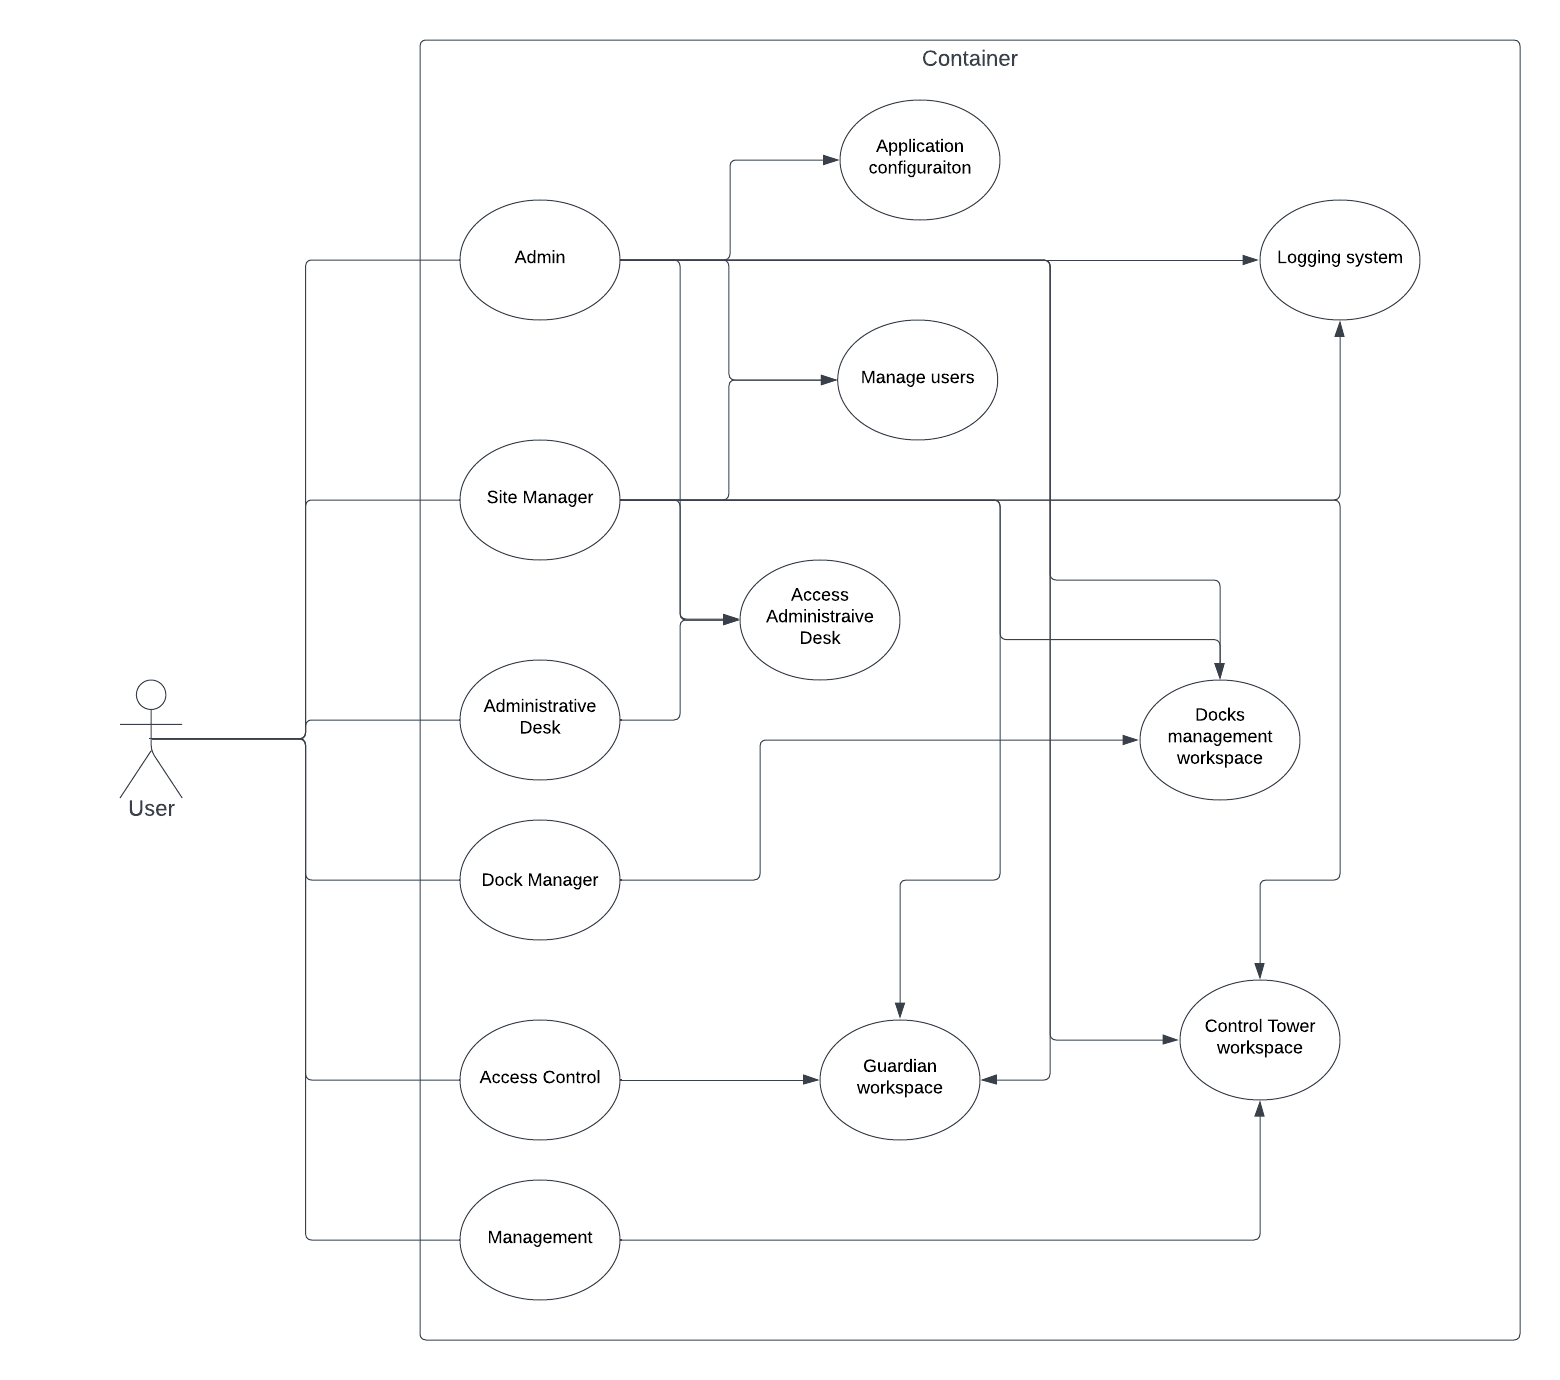
\includegraphics[width=\textwidth]{images/useCaseRoles.png}
    \caption{User Roles - Use Case}
    \label{fig:useCaseRoles}
\end{figure}

So we had to change this architecture to be able to manage users and their roles, but also
keep the old behaviour the same.

One of the major points for adding the user management system was to make it
possible to manage the workspaces of users, by having them manageable by roles
and roles being owned by users.

The roles came with access to their right workspaces as shown in the figure
\ref{fig:useCaseRoles} and the user management system was built around this system to
move from a sites only managed system to a system where users get to manage multiple
modules within the workflow.

The change from the old system to the new system came with a big migration of the backend
services and controllers.

\begin{figure}[!ht]
    \centering
    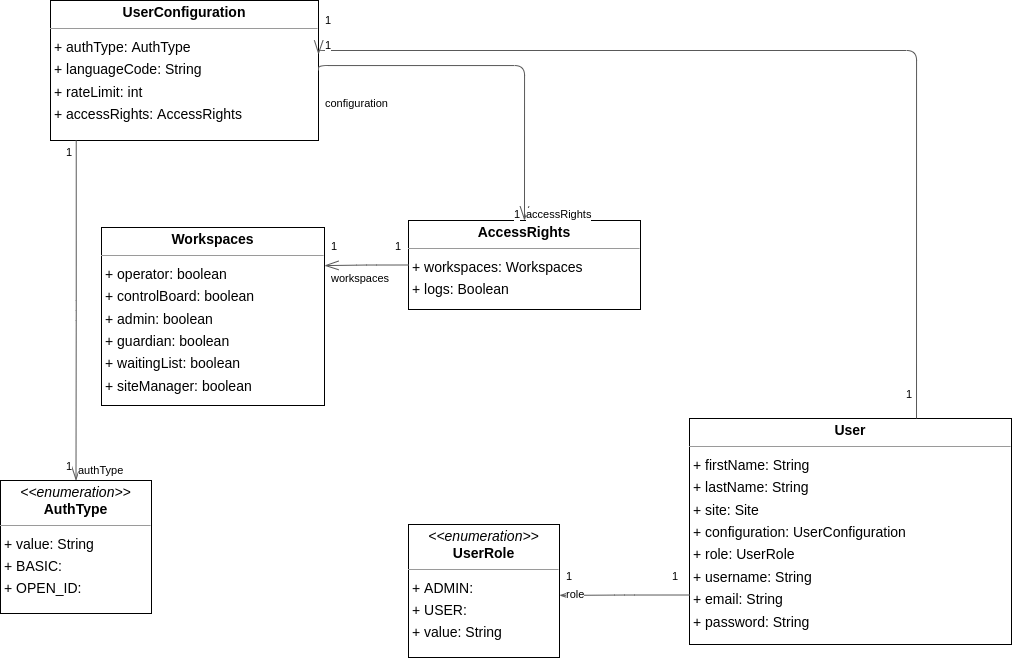
\includegraphics[width=1\textwidth]{images/userClass.png}
    \caption{User Class Diagram}
    \label{fig:userClass}
\end{figure}

First of all, the we migrated the old User class to the Site class, then we added the new
User class to the backend and it came in with the following fields and dependencies as shown
in the figure \ref{fig:userClass}.

So with the swap happening to the User class, we had to change the authentication and
authorization system to use the new User class.

During this update, we also had a big change in the backend services and controllers.
We had to automatically role back to anything that using Site or let's say the old User 
class to the be mapped to Site.

Then as Site was part of the User now, within it fields, we had to enforce a new model 
on the User authentication details, shifting from the default username only offered
by the Spring Security authentication filter, to a UserDetails that contained multiple 
data important to details to handle the requests, which was:
\begin{itemize}
    \item Username
    \item Workspaces
    \item Role
    \item Site
\end{itemize}

With this change, it made it possible to handle the change inside the controllers and
backend a more streamlined activity, which relied on a small swap of how the Site 
class was imported within those requests for handling.

\begin{sidewaysfigure}[!htpb]
    \centering
    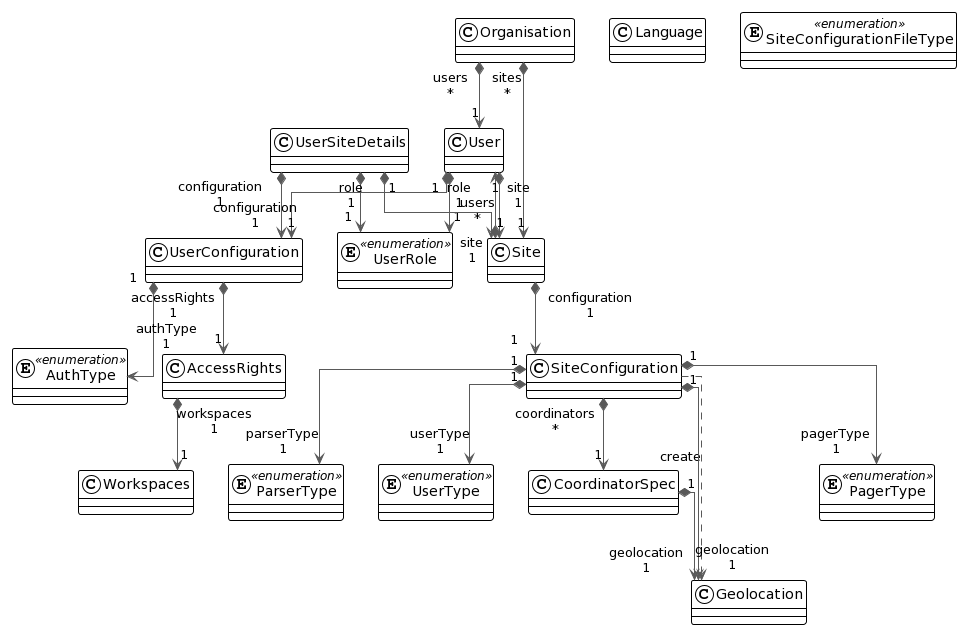
\includegraphics[width=\textwidth]{images/package.png}
    \caption{Class diagrams on User package}
    \label{fig:cd_entities}
\end{sidewaysfigure}

Finally with this change, we ended up with a new relationship between the entities
within the system, being compiled to the diagram in figure \ref{fig:cd_entities}

With this new system it's clear that there's a shift from the central system
that is the Site to the User being the cental system of managing the relationship
between the different parts.

\subsection {Refactoring}

So before beginnig a full refactoring of the existing code base, we had to do some migrations
specifically on the existing NodeJs code started to get a bit annoying to maintain, and
started to be a problem for implementing a multi-module build system, the multi-module build
system is a build which relies on having all the different modules in the same project,
which could make the development process a bit more easier to maintain. And as majority
of the build system is in Java, and which has a strong build system already in place.

So we opted to migrating the existing the NodeJS code to Java, and this was done by
rewriting the existing modules fully in Java, and then adding the new modules to the
existing multi build project.

For the refactoring of the codebase, we didn't manage to implement it yet, but we
were able to get a good idea of what the changes would look like.

Firstly this will be a big change in the backend's codebase, as it would be reworked
fully from the base up. Meaning that we go through the following:
    \begin{itemize}
        \item Implement tests for all the existing code
        \item Rework the backend architecture to be more modular and uniform
            as a monolith, that's more oriented to a reactive architecture
        \item Choose the matching framework for the new architecture
        \item Implement the reworked architecture
        \item Work on JVM optimization options
    \end{itemize}

So as of the current time, the existing backend is still missing tests 
there are tests that are currently covering around 10\% of the codebase.
And with such a huge code base, implementing tests for existing code can
be quite the challenge as it's missing documentation.
This step is really important, as it's would allow to make sure that the
existing behaviour remains intact after the refactoring.

Next the rework of the backend architecture, the new architecture is aimed to
be based on the reactive paradigm, which can give us a loosely coupled
backend, which is a good thing for the longivity of the project.
Also it would be more matching for the problem domain, as it's more focused
on having to deal with real-time data, and not just static data.
So it relies on a events reacting to the data change, which calls for a 
paradigm that oriented for a event-driven architecture.

The JVM optimization options are a bit of tricky ones, as they are
based on the VM options, and the VM to go with either stick to a Java Virtual Machine
(JVM), Spring boot combination or opt for something that is more lightweight and faster
with booting like a GraalVM and Quarkus combination.
GraalVM is a high-performance JDK distribution designed for a more optimized memory usage,
and a accelerated execution time \cite{grl_jvm}.
Quarkus is a Java EE micro-framework that is designed to be used as a lightweight
container for Java EE applications, so it's a rather more optimized option to be cloud
hosted.
As of the current time, we still not decided on which option to opt for yet.
But with the current infrastructure that is relying on more dockerized containers,
that are hosted on a cloud provider, the latter option does sound like a better one
but that would be a huge change from the current existing code base.
